\chapter{Design}
	\label{chap:methodology}
		
	%The university has subscriptions to a vast number of major academic journals spanning a wide range of subject areas. By accessing the internet from a university network connection (Eduroam or Ethernet), the paywalls of many journals will simply vanish without any need for login credentials.

	\section{Overview of Application}
	%	When you are working from outside of the university then connecting to an on campus machine via remote desktop (RemoteDesktopProtocol, TeamViewer, ect) or via port forwarding (ssh, ssh tunnel, ect) can allow you to access papers that would otherwise be behind a paywall. 
		
	%	If you do not have individual access to a machine that is exposed for ssh on the university network you can always use the computers in Linux Lab CF204\footnote{One caveat of using computer lab machines for remote tunnelling is that a environmentally conscious student who has worked late in the computer lab might choose to switch off the machine you were using...} for the purpose of setting up an ssh port tunnel to proxy your internet through. These machines have fixed IPv4 addresses and respond to ssh using your student account credentials. While in use your internet will be routed\footnote{Painfully slowly.} to the university and then out to the internet, granting you transparent access to journals without a paywall.
	The application has three main segments. These segments are a game area, a learning area and an exploring area. Each area's intension is to help support the user learning and understanding of the different machine learning models using a blend of exploration, fun and interactivity as well as a more traditional teaching a learning style of quizzes and learning reading material. Although each segment has its core task, together they help give the user a rounded learning experience while creating gamification incentives to come back and use the application some more.
	
	With the application being about the user interacting with data, and placing (splashing) the data points around a game board, we decided upon the title "Data Splash". With the title 'Data Splash" agreed upon, a beach and sea themed colour pallet got chosen. The pallets colours contained blue, yellow, turquoise and orange. However, additional colours got used to aid the colour pallet selected, and these colours involved grey and red.
	
	All the screens had a similar layout, with a title banner image at the top, the content in the middle and the buttons in the bottom general area. The only screens that are different are the main menu screen and the coming soon splash screen. The main menu did follow a similar structure, but the main content was the buttons, which get presented in a horizontal stage manner (see fig: ??).
	
	Whenever a model or educational content got made available to the player, this content was the main focus to the screen. Therefore always making sure that the user's attention was on interacting with the model or learning about them. Unless like in the Free Play area, both learning and model interaction was available, equal weighting occurred given to allow focus on interacting and learning about the machine learning models.
		
	%\subsection{Design}
	
	%\begin{figure}[t]
	%	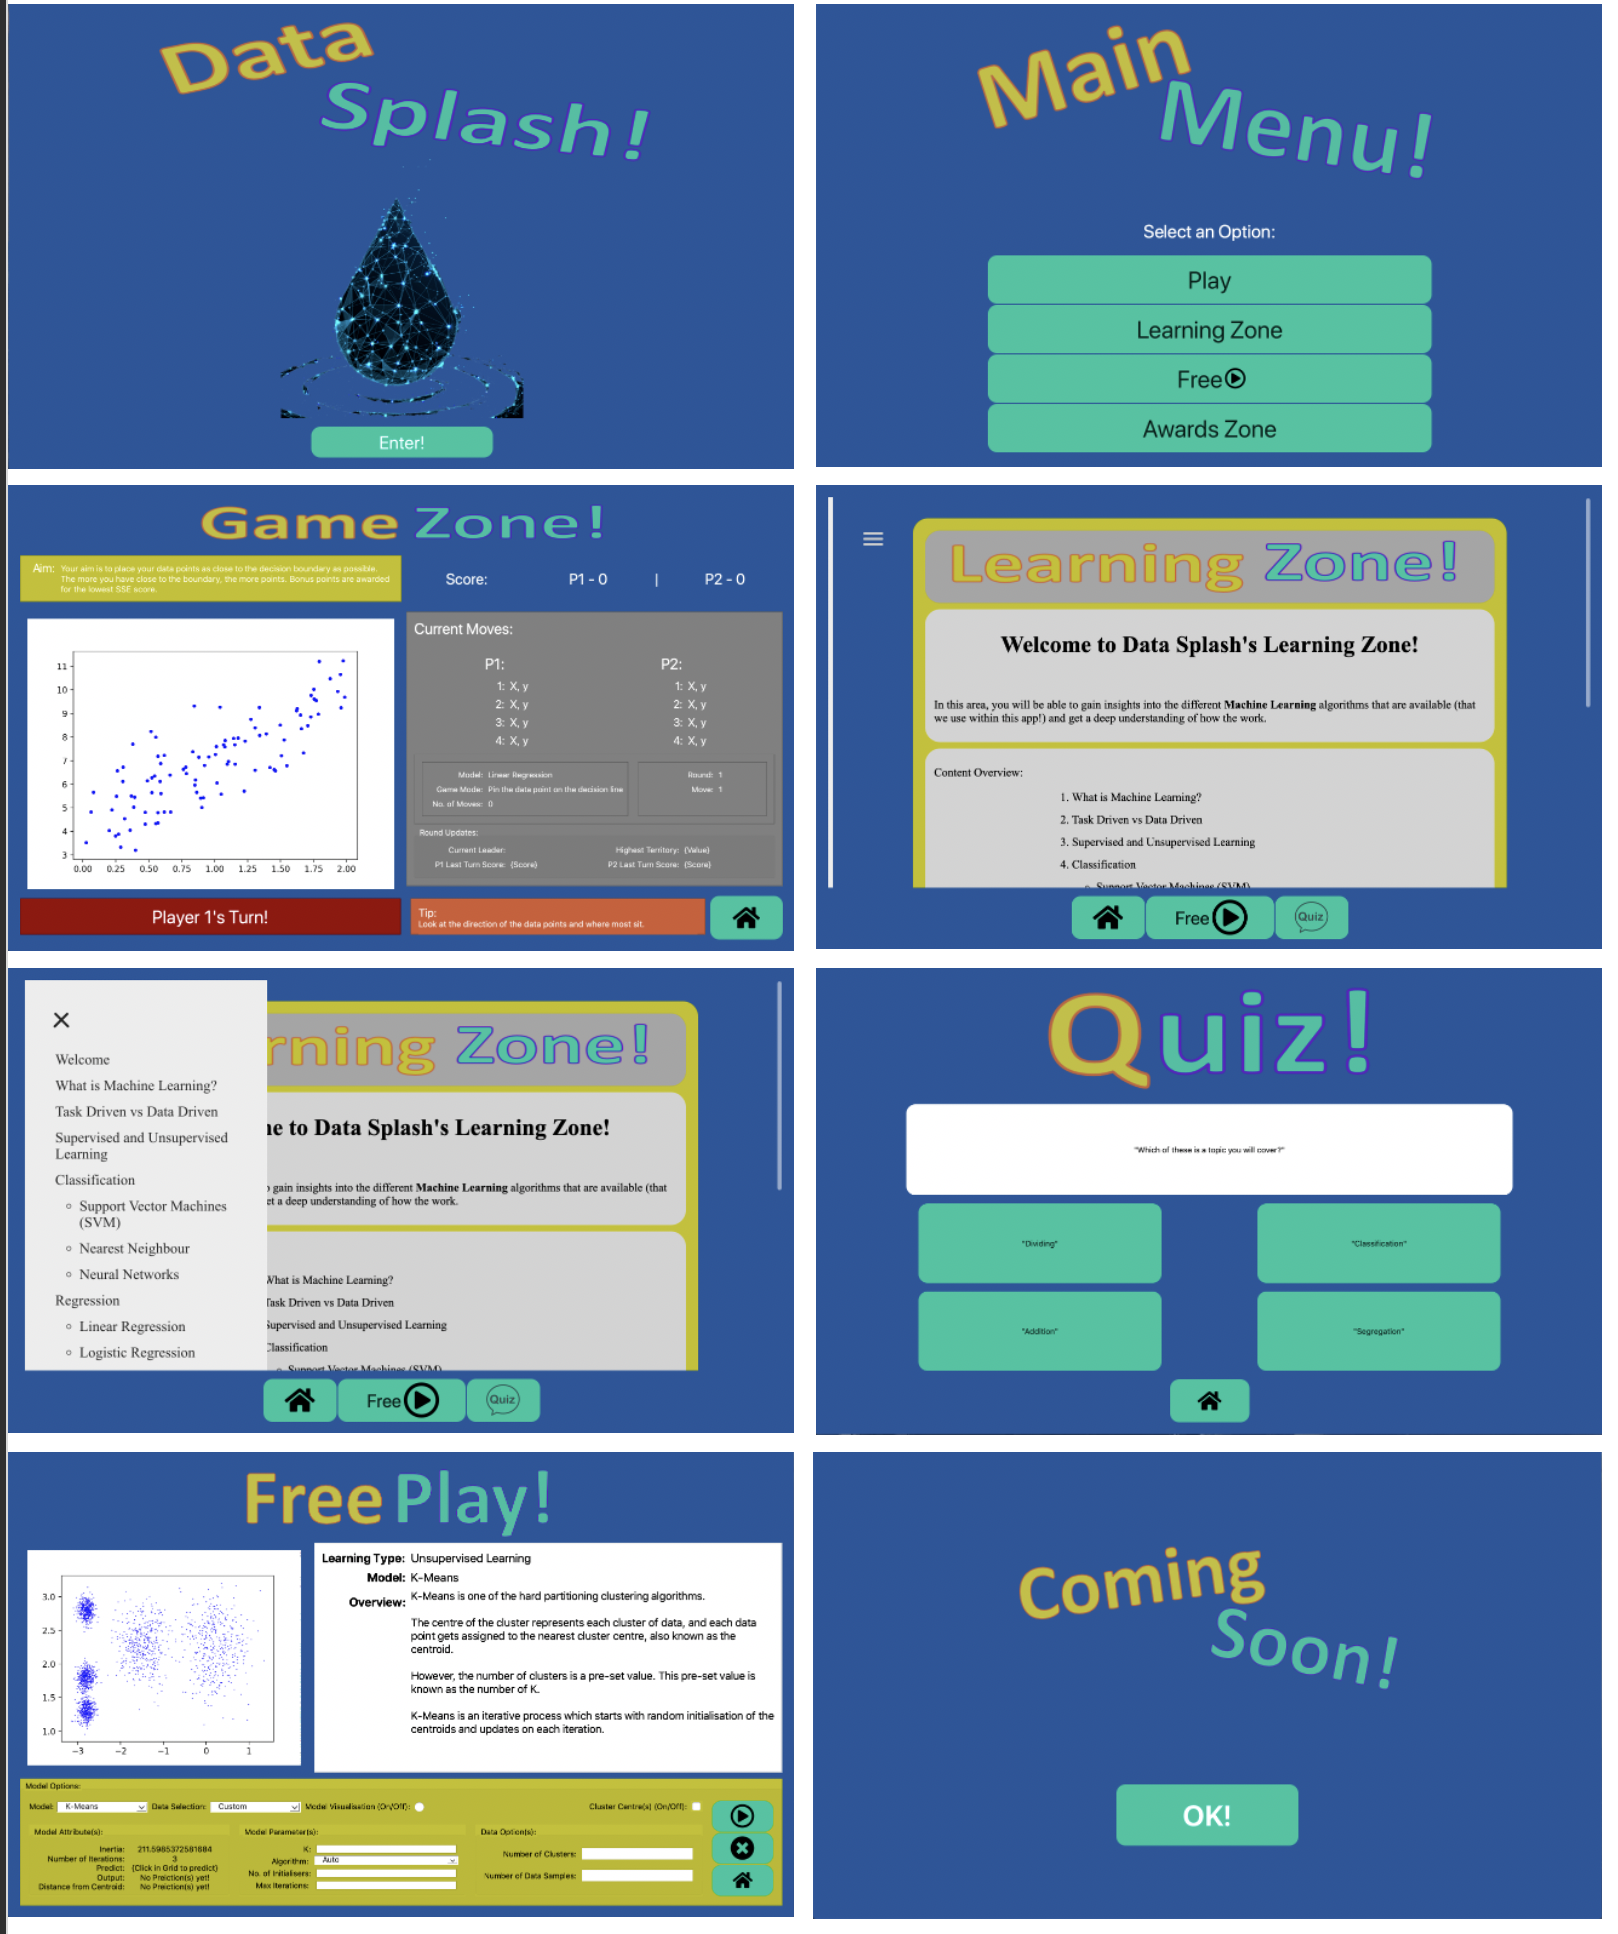
\includegraphics[width=15cm]{graphics/ui_screens.png}
	%	\caption{Each screen available within the application.}
	%	\label{fig:ui_screens}
	%\end{figure}
	
	
	
		
		
		
	\section{Overview of Specific Game Components}
		\label{sec:overview_game_components}
		
	
	\subsection{Main Menu}
	\begin{figure}[t]
		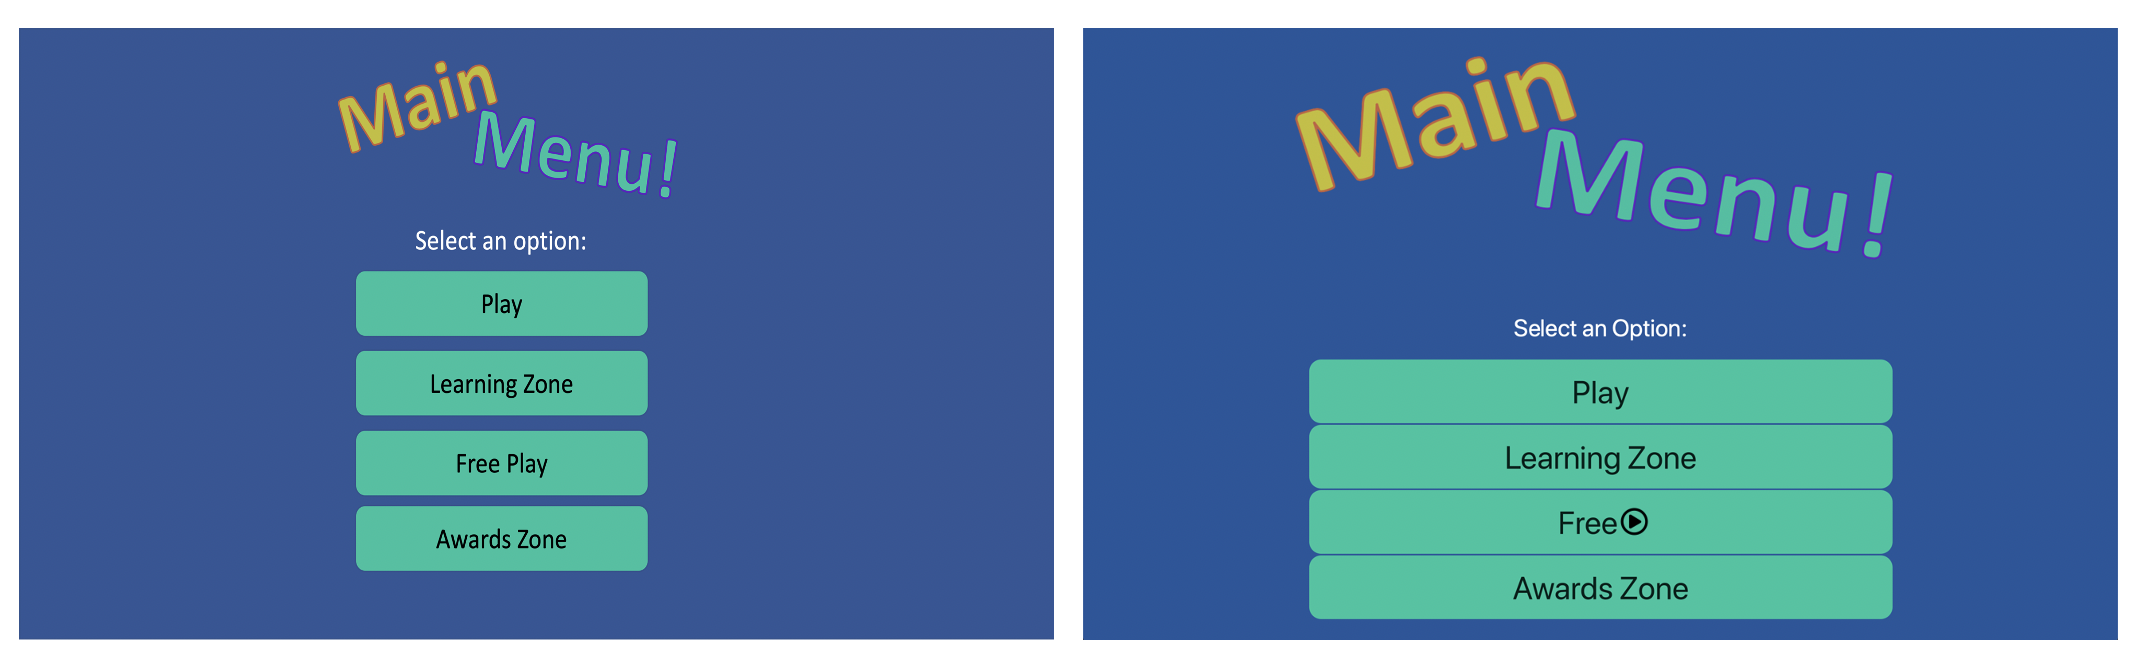
\includegraphics[width=15cm]{graphics/main_menu.png}
		\caption{A comparison of the main menu's designed screen UI and the final implmented UI.}
		\label{fig:ui_mm}
	\end{figure}
	
		
	\subsection{Game Arena}
	
		The 'Game Zone' was the critical area that intended to use game mechanics, and gamification, to help drive the learning of the different machine learning models. The game zone is an area that allows one on one (player vs player) game action. The game gets conducted over three rounds, with each game round having a random model generated for the players to interact. At the time of writing this report, the available models for the game zone are Linear Regression and K-Means. A Neural Network got implemented with game mechanics, but due to time restrictions, we were unable to add them to the application in time. As the research suggested, having a competitive nature to the game creates desired external motivation for the player to learn more about the ML models, to be able to have a better chance of winning. A running score is presented to the players to let them know who won the previous round and who is currently winning. The multiple forms of game stats allow the players to have an idea of what is needed to win the game potentially through using sport like game mechanics to add the layer of progress updates continuously, to create that sense of competitiveness and external motivation. Even though there were only two models implemented fully into the game, these models offered several different gaming outcomes. For example, each model had multiple datasets which would get selected at random. In terms of K-Means, a random dataset would get generated each time or a preselected dataset, but the k value would change and be a random number. So even though the dataset was a k value of 2, the challenge would be added by not knowing what k value was given to the model for the user to predict the centroid value. 
		
		We selected K-Means and Linear Regression to be implemented first due to them both having a similar game mechanic intention. Linear Regression was using the SSE metric value as the deciding factor to determine the game's winner, while K-Means was using the model's metric value of the euclidean distance to do the same thing. The neural network uses a territory-based mechanic, and this intention was to add variety in not only the models but the game times. Challenging the players understanding of how different models work.
		
		With having multiple models available, as well as getting the models and their datasets randomly selected each time, this allows the game to feel fresh each time and not have a set pattern of motions. Therefore, by creating a sense of game mode uncertainty or randomness will keep things fresh. Thus, ultimately making sure that a critical mechanic of gamification, which is replayability, be achieved.  
		
		There were intentions for the Learning Zone to also provide example code for the user, after specific gamification actions, for example getting full marks in the quiz, were completed as bonus rewards. The intention of this was to allow the users to not only learn about the code but also see the code, to help see the mechanics in it. However, due to time restrictions and certain gamification features not being implemented, this additional feature was not added at this point.
		
		\begin{figure}[t]
			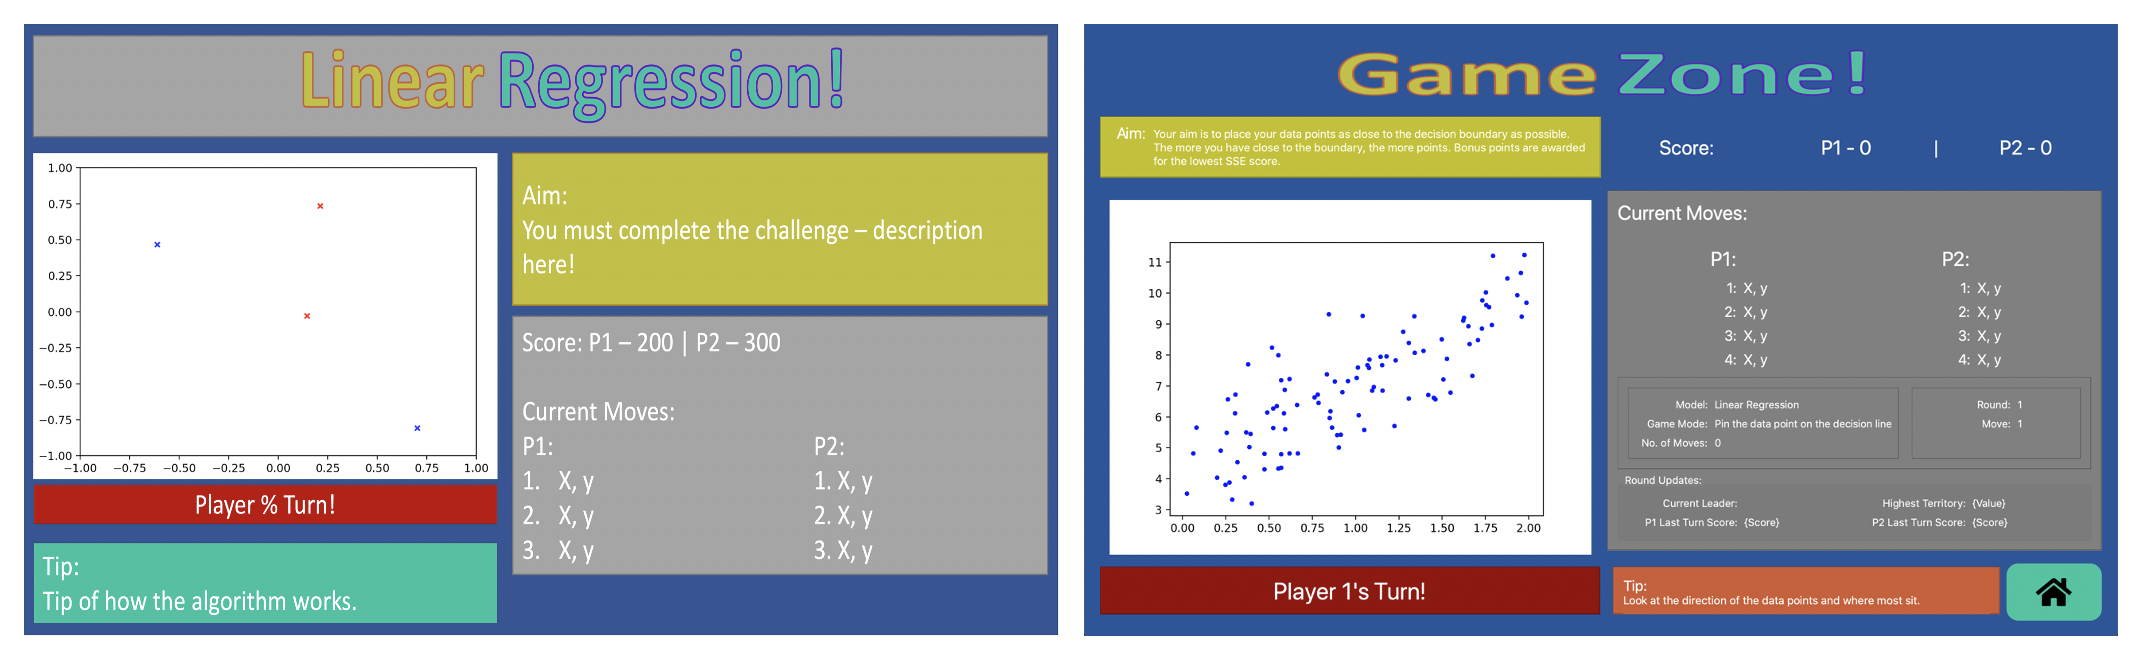
\includegraphics[width=15cm]{graphics/game_zone.png}
			\caption{A comparison of the game area's designed screen UI and the final implmented UI.}
			\label{fig:ui_ga}
		\end{figure}
	
	\subsection{Learning Zone}
	
	The learning zones aim is for the user to do the principal amount of learning about the different machine learning models. The main content gets presented to the user by using a web browser widget. This widget would link to a multipage HTML website that holds all the content about the different models with pictures. We decided to use this combination as it allowed us to update the learning content and add new content as we went along, enabling the main functionality not get affected. Also, it avoided unnecessary long developing time, because of the updates and the new content, forcing the redesign of the game screen. 
	
	With the teaching and learning getting conducted through text and images on the webpages, we decided to add a quiz. The quiz was to allow the user to assess how much they have learnt. A useful tool used by teachers to evaluate students learning is different questioning techniques. In an attempt to allow the users to test their subject knowledge, but keeping everything in a game-like manner, a quiz was implemented. The quiz, with not only challenging the user but also offers an overall score allowing the user to know how they did and will enable a form of competition to happen and also let the use sense a way of progression by observing their performance improving.
	
	An option available to the user is not only to quiz themself but also to have the ability to go straight to the Free Play area. When the user selected this option, the model that the user has been learning about will be preloaded into the screen, allowing them to be able to interact with it. We decided to do this as although you can learn a lot about a topic by reading about it, an effective way to truly learn about something is to be able to interact with it and see what is happening by, in essence, trying to break it in a sort of way.
	
	\begin{figure}[t]
		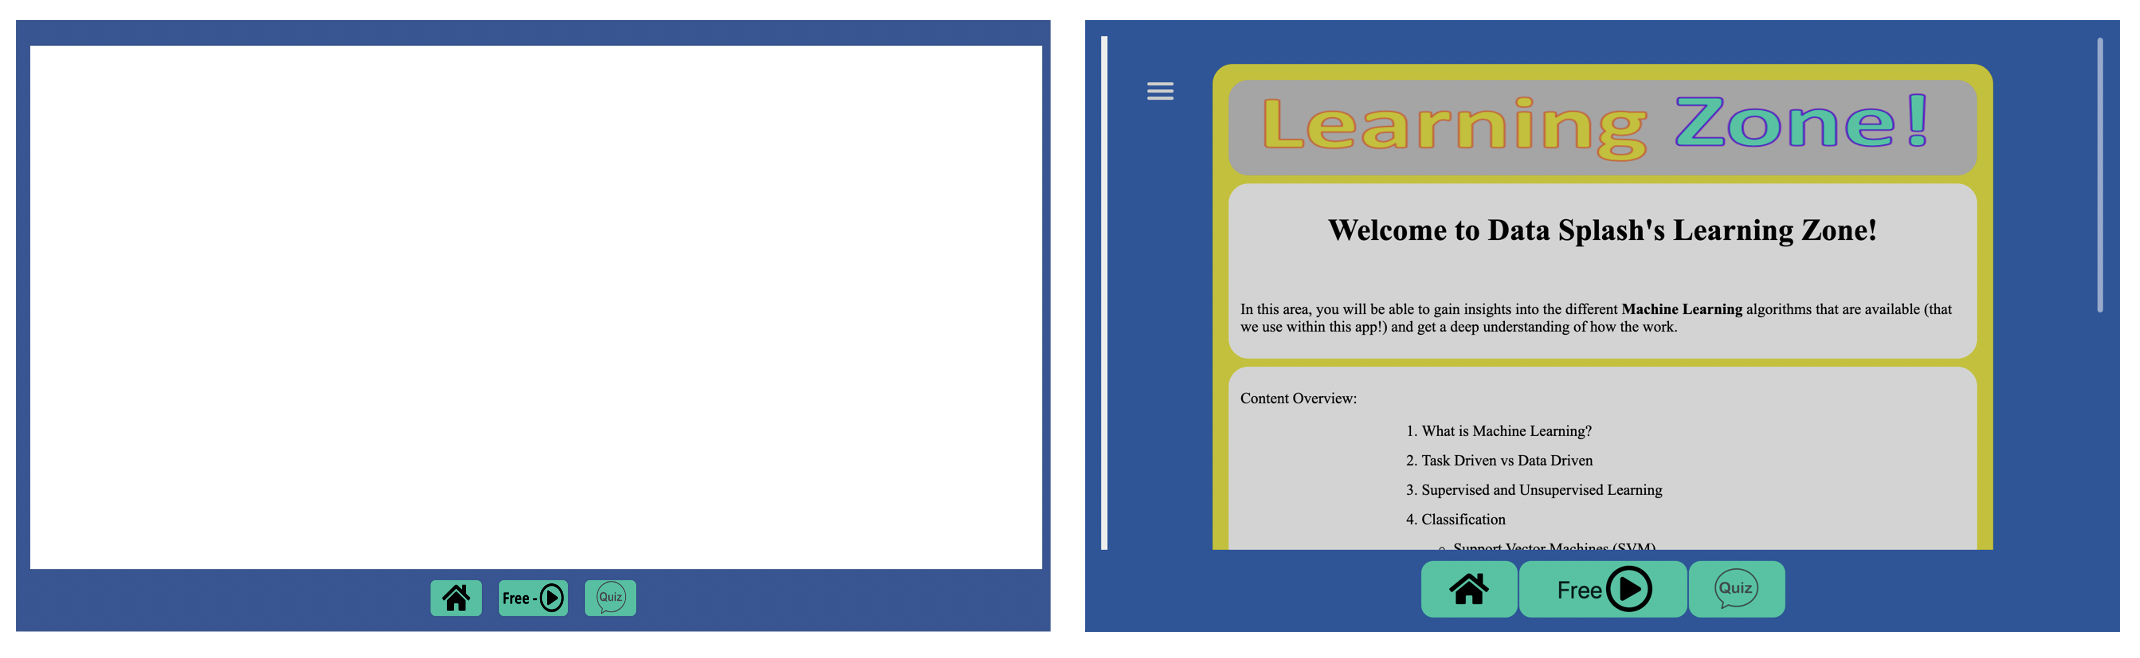
\includegraphics[width=15cm]{graphics/learning_zone.png}
		\caption{A comparison of the learning zone's designed screen UI and the final implmented UI.}
		\label{fig:ui_lz}
	\end{figure}
	
	\subsection{Free Play}
	
	The free play area is where the serious gamification style gets implemented. This area intends to allow users to be able to interact with the ML models. Initialise not only the models but also set the type of data they want to have displayed and even add additional data points. By allowing the user to add extra data points to the existing data, it will update the model and, for example with Linear Regression, will show to the user, how the additional data points will affect the model's decision making.
	
	\begin{figure}[t]
		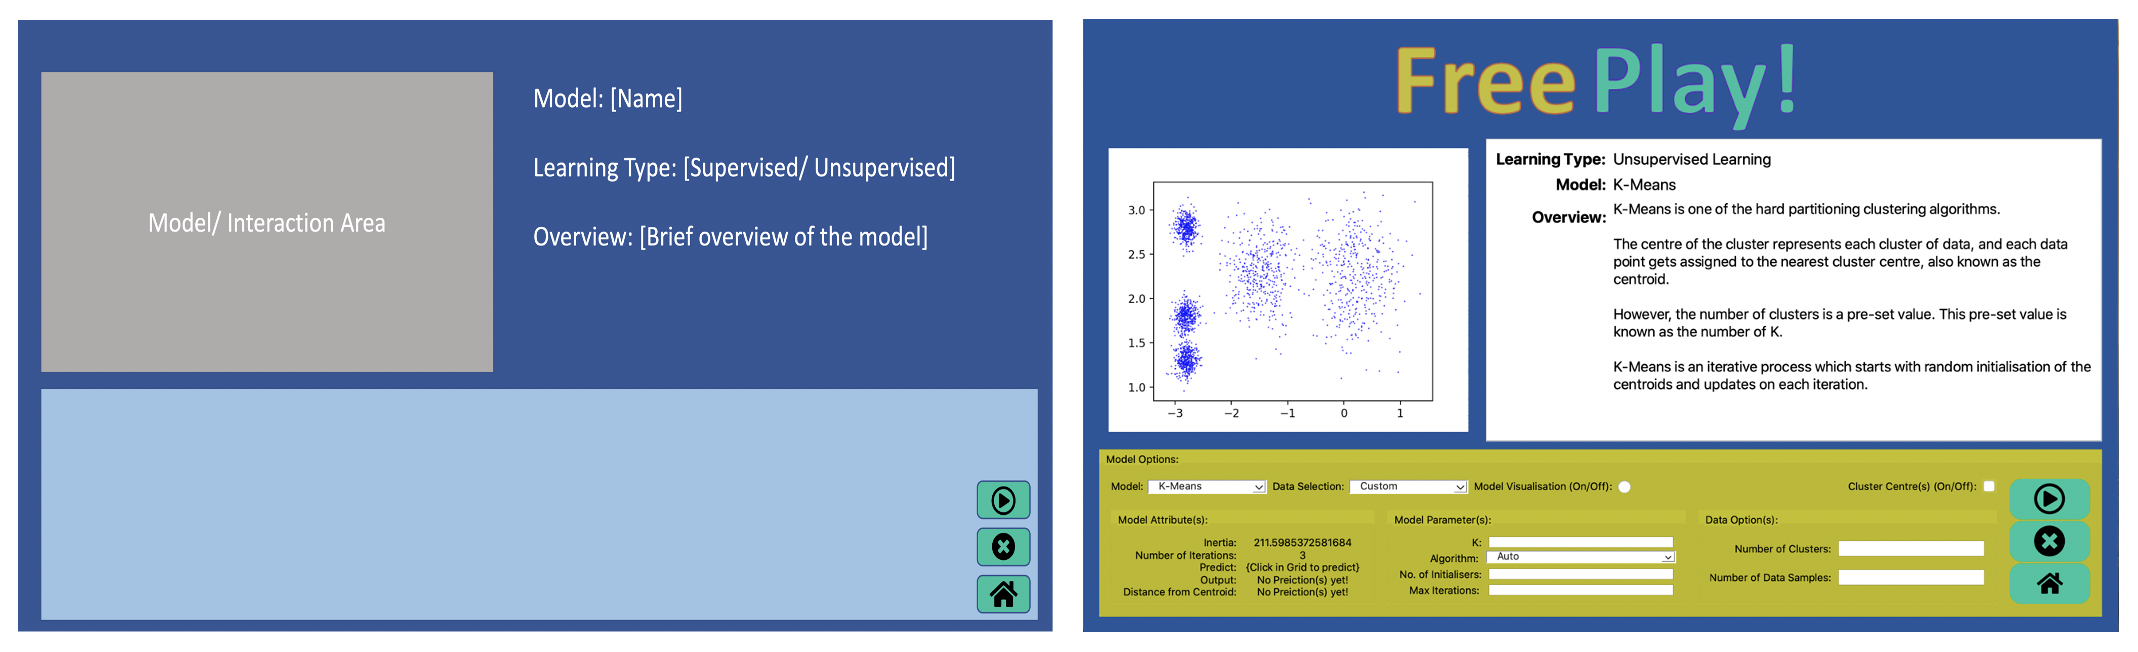
\includegraphics[width=15cm]{graphics/free_play.png}
		\caption{A comparison of the free play's designed screen UI and the final implmented UI.}
		\label{fig:ui_fp}
	\end{figure}
	
	The most interactive model's within the FP area, at current, are the models Linear Regression, K-Means, LDA and Neural Networks. However, the models GMM and SVM are also available, but with less interactivity as the others. K-Means allows the user not only to select different data sample but also select how many clusters they want the dataset to have, but also independently change the k value of clusters. We decided upon this feature to allow the user to see, knowing how many k clusters the dataset has, to see by changing the algorithms k value how is that then affected on the dataset with its outcome. The user can click within the Matplotlib widget and see what the data points prediction values are as well. We decided to use a click in the widget functionality, as we believed having the user input x and y coordinates would make the UI look cumbersome and add unneeded fiddliness for the user, trying to figure out the exact values they want. Linear regression allows the player to be able to make predictions, as well as additional data points allowing them to see how the data can be altered and manipulate and what implications that has on the models fitting. However, Linear Regression does not provide as much control for the intricacies of the model compared to K-Means, but it does offer the parameters and outputs that the model has. For example, the intercept and the coefficients to the model. Neural Networks offer slightly less control to the user compared to the other two, but more than LDA but both of them have fully interactive models. SVM and GMM, on the other hand, do not. GMM allows the user to switch its predictions on and off, but SVM just shows the models predictions. These got implemented to help with understanding the content from the learning zone, but we decided to focus on the other models due to them having more game-like features to get used in the game area.
	
	
	
	
	\subsection{Awards Zone}
	
	
	The achievement area has just a title, coming soon image and a button. Once the button gets pressed, it will return the player to the main menu. This area intention was to be the central hub of where all the gamification elements of badge unlock and progress, would be displayed to the user, giving them instant feedback on unlocked prizes and game modes,  as well as hints on what to do to unlock additional features. However, due to time restrictions, this was unable to be implemented within the application. The idea was to allow the users to see how or what affects the models, from little changes to significant changes like changing the number of clusters in k-Means or the main algorithm being used to fit the clustering data. The intention was to allow the user to get hands-on with the different models, to see what they have learnt from the learning zone in motion, and also try out strategies for the game zone. 
	
	The models had three data settings, a custom one and two pre-generated datasets. The pre-generated data sets allow the user to be able to change the features that are used, assigning news features to the X and y-axis.
	
	\begin{figure}[t]
		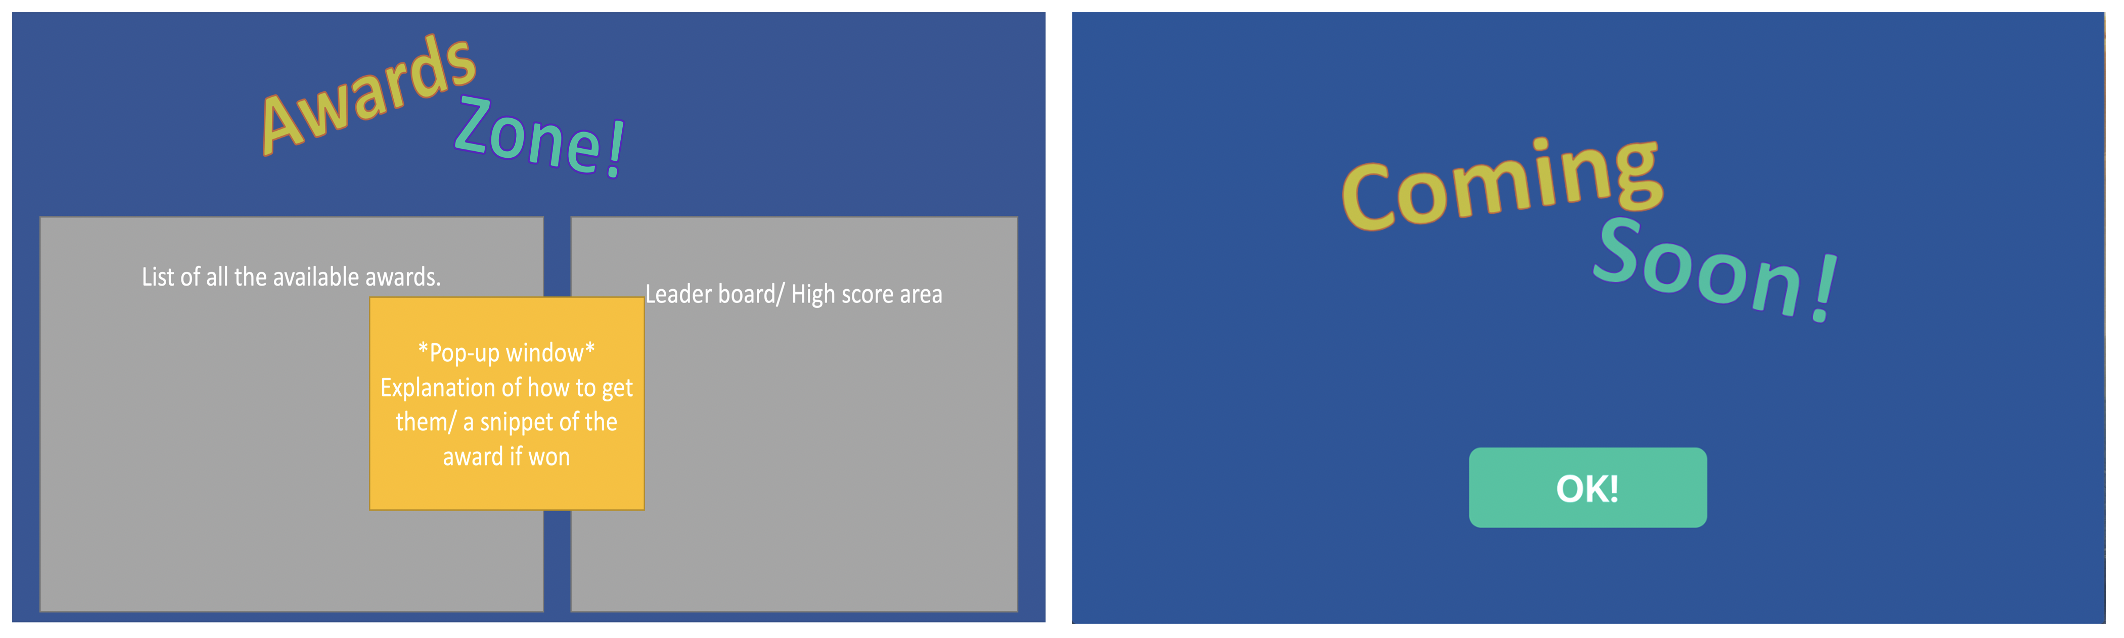
\includegraphics[width=15cm]{graphics/awards_zone.png}
		\caption{A comparison of the awards zone's designed screen UI and the final implmented UI.}
		\label{fig:ui_az}
	\end{figure}
	
			
	\section{Evaluation of Application}
		\label{sec:app_evaluation}
	
		To gain a deeper understanding of the application, for its effectiveness and the general overall thoughts from other peoples views, a user study got conducted. The user study involved participants in interacting with the application and then fill in an online questionnaire about what they thought of it. However, due to the coronavirus pandemic, the study got done all remotely.
		
		The user study involved [number] of participants and got done in a quantitative style, using questionnaires of a range scale. This style of questions got decided upon due to the inability to ask the candidates follow-up questions. The participants got asked to install the application and then spend a minimum of 20 minutes interacting with it. After they had spent a minimum of 20 minutes on the application, they then needed to complete a questionnaire. The questionnaire consisted of [number of] questions with the questions either a range option style question of 1 to 5 or a short paragraph explanation. The questionnaire got conducted using Google Forms, which allowed us to have all the responses appear in a spreadsheet. Therefore, allowing reflection on the user's opinions more accessible.
		
		[What are the results?]
		